
\section{Work and Power\footnote{
1990-93 Dept. of Physics and Astronomy, Dickinson College. Supported by FIPSE
(U.S. Dept. of Ed.) and NSF. Portions of this material have been modified locally
and may not have been classroom tested at Dickinson College.
}}

\makelabheader %(Space for student name, etc., defined in master.tex or labmanual_formatting_commands.tex)

\textbf{Objectives }

\begin{itemize}
\item To extend the intuitive notion of work as physical effort to a formal mathematical
definition of work as a function of force and distance. 
\item To understand the concept of power and its relationship to work.
\end{itemize}
\textbf{Apparatus }

\begin{itemize}
\item 5.0 newton spring scale 
\item Wooden block with hook 
\item Variety of masses
\end{itemize}
\textbf{The Concept of Physical Work }

Suppose you are president of the Richmond Load 'n' Go Co. A local college has
three jobs available and will allow you to choose which one you want before
offering the other two jobs to rival companies. All three jobs pay the same
amount of money. Which one would you choose for your crew?

\vspace{0.3cm}
{\par\centering 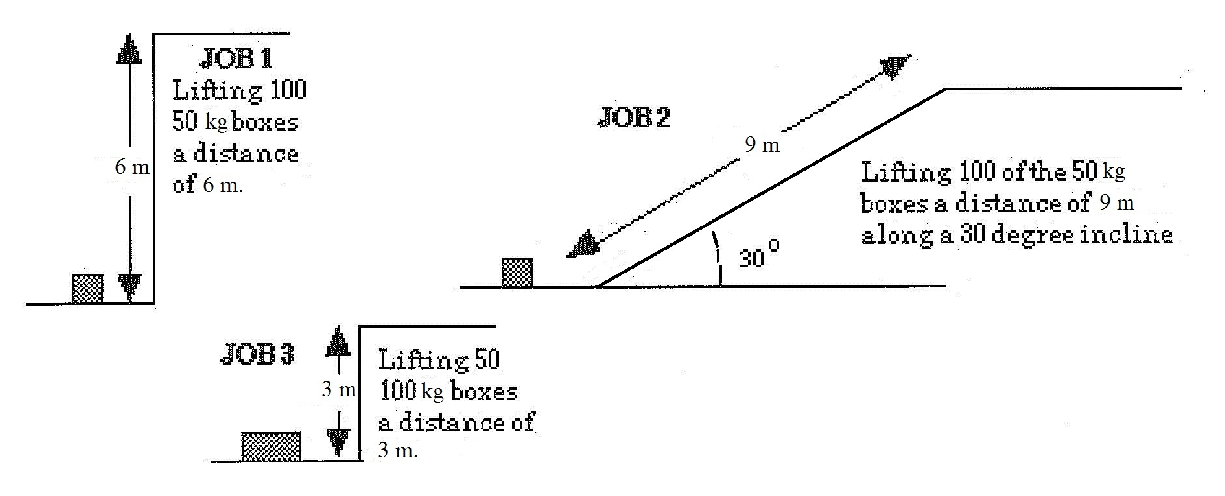
\includegraphics[width=6.2in,]{work_power/work_power_fig1s.eps} \par}
\vspace{0.3cm}

\textbf{Activity 1: Choosing Your Job }

Examine the descriptions of the jobs shown in figure above. Which one would
you be most likely to choose? Least likely to choose? Explain the reasons for
your answer.
\vspace{30mm}

You obviously want to do the least amount of work for the most money. Before
you reconsider your answers later in this unit, you should do a series of activities
to get a better feel for what physicists mean by work and how the president
of Load 'n' Go can make top dollar.

\vspace{0.3cm}
{\par\centering 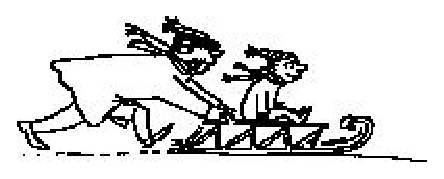
\includegraphics{work_power/work_power_fig2.eps} \par}
\vspace{0.3cm}

In everyday language we refer to doing work whenever we expend effort. In order
to get an intuitive feel for how we might define work mathematically, you should
experiment with moving your textbook back and forth along a table top and a
rougher surface such as a carpeted floor.

\textbf{Activity 2: This is Work!} 

(a) Pick a distance of a meter or so. Sense how much effort it takes to push
a heavy book that distance. How much more effort does it take to push it twice
as far? 
\vspace{20mm}

(b) Pile another similar book on top of the original one and sense how much
effort it takes to push the two books through the distance you picked. Comment
below.
\vspace{20mm}

(c) From your study of sliding friction, what is the relationship between the
mass of a sliding object and the friction force it experiences? On the basis
of your experience with sliding friction, estimate how much more force you have
to apply to push two books compared to one book.
\vspace{20mm}

(d) If the ``effort'' it takes to move an object is associated
with physical work, guess an equation that can be used to define work mathematically
when the force on an object and its displacement (i.e., the distance it moves)
lie along the same line.
\vspace{20mm}

In physics, work is not simply effort. In fact, the physicist's definition of
work is precise and mathematical. In order to have a full understanding of how
work is defined in physics, we need to consider its definition in a very simple
situation and then enrich it later to include more realistic situations.

\textbf{A Simple Definition of Physical Work:} If an object that is moving in
a straight line experiences a constant force in the direction of its motion
during the time it is undergoing a displacement, the work done by the external
force, \( F_{ext} \), is defined as the product of the force and the displacement of the object, 
\[
W=F_{ext}\Delta x\]


where $W$ represents the work done by the external force, \( F_{ext} \) is the
magnitude of the force, and \( \Delta  x\) is the displacement of the object.
%WHY THE HECK DO WE SAY THIS:
%{\bf I WANT TO DROP THIS SENTENCE:} Work done by a force is always positive!

What if the force of interest and the displacement are in opposite directions? For instance, what about the work done by the force of sliding friction,
\( F_{f} \), when a block slides on a rough surface? The work done by the friction force is
\[
W_{f}=-F_{f}\Delta x\]
%YUCK:
%{\bf AND THIS ONE:} Work done against a force is always negative!

\textbf{Activity 3: Applying the Physics Definition of Work} 

(a) Does effort necessarily result in physical work? Suppose two guys are in
an evenly matched tug of war. They are obviously expending effort to pull on the
rope, but according to the definition of physical work, are they doing any physical
work? Explain.

\vspace{0.3cm}
{\par\centering 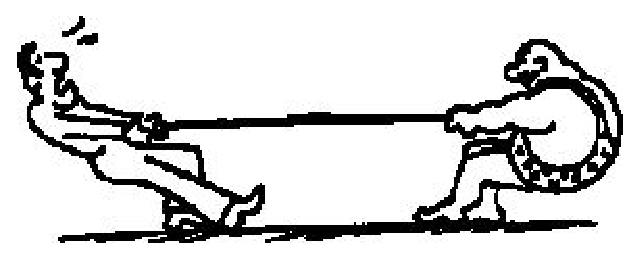
\includegraphics{work_power/work_power_fig3.eps} \par}
\vspace{0.3cm}

(b) A wooden block with a mass of .30 kg is pushed along a sheet of ice that
has no friction with a constant external force of 10 N which acts in a 
horizontal direction. After it moves a distance of 0.40 m how much work has 
been done on the block by the external force?
\vspace{20mm}

(c) The same wooden block with a mass of .30 kg is pushed along a table with
a constant external force of 10 N which acts in a horizontal direction. It moves
a distance of 0.40 m. However, there is a friction force opposing its motion.
Assume that the coefficient of sliding friction, \( \mu _{k} \), is 0.20. 

\vspace{0.3cm}
{\par\centering 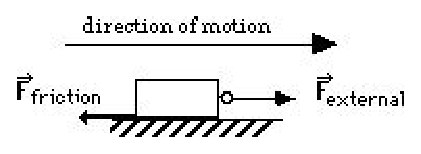
\includegraphics{work_power/work_power_fig4.eps} \par}
\vspace{0.3cm}

\begin{enumerate}
\item According to the definition of work done by a force, what is the work associated with the external force? Is the work positive or negative? Show your calculation. Note: This is the same as part (b) above.
\vspace{20mm}

\item According to our discussion above of the work done by a friction force, what is the work associated with the friction force? Is the work positive or negative? Show your calculation. (See the equation above, just before Activity 3.)
\vspace{20mm}

\end{enumerate}
(d) Suppose you lift a 0.3 kg object through a vertical distance of 1.0 m at a constant velocity.

\vspace{0.3cm}
{\par\centering 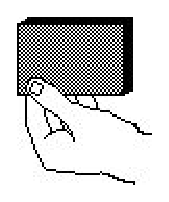
\includegraphics{work_power/work_power_fig5.eps} \par}
\vspace{0.3cm}

\begin{enumerate}
\item What is the work associated with the force that the earth exerts on the object? Is the work positive or negative? Show your calculation.
\vspace{20mm}

\item What is the work associated with the external force you apply to the object? Is the work positive or negative? Show your calculation.
\vspace{20mm}

\end{enumerate}
\textbf{Pulling at an Angle: What Happens When the Force and the Displacement
Are Not Along the Same Line? }

Let's be more quantitative about measuring force and distance and calculating
the work. How should work be calculated when the external force and the 
displacement of an object are not in the same direction?

\vspace{0.3cm}
{\par\centering 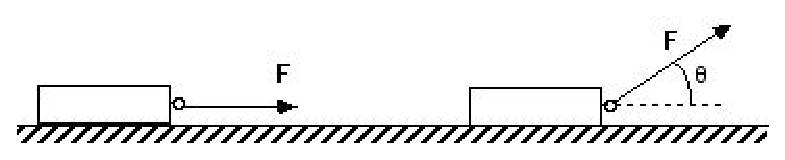
\includegraphics{work_power/work_power_fig6.eps} \par}
\vspace{0.3cm}

To investigate this, you will use a spring scale to measure the force necessary
to slide a block along the table at a constant speed. Before you make your simple force measurements, put some weights on your block so that it slides along a smooth surface at a constant velocity even when it is being pulled with a force that is 30 or 60 degrees from the horizontal.

\textbf{Activity 4: Calculating Work} 

(a) Hold a spring scale horizontal to the table and use it to pull the block 
(with 500 grams on it)
a distance of 0.5 meters along the horizontal surface in such a way that the
block moves at a constant speed. Record the force in newtons and the distance
in meters in the space below and calculate the work done on the block in joules.
(Note that there is a special unit for work, the joule, or J for short. One 
joule is equal to one newton times one meter, i.e., J = N\,m.)
\vspace{20mm}

\newpage
(b) Repeat the measurement, only this time pull on the block at a 30\( ^{\circ } \) angle with respect to the horizontal. Pull the block at about the same speed. Is the force needed larger or smaller than you measured in part (a)?
\vspace{20mm}

(c) Repeat the measurement once more, this time pulling the block at a 60\( ^{\circ } \) angle with respect to the horizontal.  Pull the block at about the same speed as before.
\vspace{20mm}

(d) Assuming that the actual physical work done in part (b) is the same as the
physical work done in part (a) above, how could you enhance the mathematical
definition of work so that the forces measured in part (b) could be used to
calculate work? In other words, use your data to postulate a mathematical equation
that relates the physical work, $W$, to the magnitude of the applied force, $F$,
the magnitude of the displacement, \( \Delta  s\), and the angle, \( \theta  \),
between $F$ and \( \Delta  s\). Explain your reasoning. Hint: sin 30\( ^{\circ } \)
= .500, sin 60\( ^{\circ } \) = .866, cos 30\( ^{\circ } \) = .866, cos 60\( ^{\circ } \)
= .500.
\vspace{30mm}

\textbf{Work as a Dot Product }

Review the definition of dot (or scalar) product as a special product of two
vectors in your textbook, and convince yourself that the dot product can be
used to define physical work in general cases when the force is constant but
not necessarily in the direction of the displacement resulting from it. 
\[W={\bf F}\cdot {\bf \Delta s}\]


\textbf{Activity 5: How Much Work Goes with Each Job? }

(a) Re-examine the descriptions of the jobs shown in the figure on the first
page of this experiment. What is the minimum physical work done in job 1?
\vspace{20mm}

(b) What is the minimum physical work done in job 2? Get the angle right. 
Remember that even though you are going up an inclined plane, the force you 
exert to counteract gravity is straight upward.
\vspace{25mm}


(c) What is the minimum physical work is done in job 3?
\vspace{25mm}

(d) Was your original intuition about which job to take correct? Which job 
should Richmond Load 'n' Go try to land?
\vspace{20mm}

\textbf{The Concept of Power} 

People are interested in more than physical work. They are also interested in
the rate at which physical work can be done. Average power, \( \left\langle P\right\rangle  \),
is defined as the ratio of the amount of work done, \( \Delta  W\), to the
time interval, \( \Delta  t\), it takes to do the work, so that
\[
\left\langle P\right\rangle =\frac{\Delta W}{\Delta t}.\]


Instantaneous power is given by the derivative of work with respect to time,
or
\[
P=\frac{dW}{dt}.\]


If work is measured in joules and time in seconds then the fundamental unit
of power is in joules/second where 1 joule/second equals one watt. However,
a more traditional unit of power is the horsepower, which represents the rate
at which a typical work horse can do physical work. It turns out that \textit{1
horsepower (or hp) = 746 watts = 746 joules/second}.

Those of you who are car buffs know that horsepower is a big deal in rating
high performance cars. The hp in a souped-up car is in the hundreds. How does
your stair climbing ability stack up? Let's see how long it takes you to climb
the two stories of stairs in the science center.

\textbf{Activity 6: Rate the Horsepower in Your Legs} 

(a) Determine the time it takes you to climb the two flights of stairs in
the science center. Then measure the height of the climb and compute the work
done against the force of gravity.
\vspace{25mm}

(b) Compute the average power, \( \left\langle P\right\rangle  \), you expended
in hp. How does this compare to the horsepower of your favorite automobile?
If you're not into cars, how do you stack up against a horse?

